\documentclass[a4paper]{article}

\def\npart{IB}

\def\ntitle{Markov Chains}
\def\nlecturer{G.\ R.\ Grimmet}

\def\nterm{Michaelmas}
\def\nyear{2017}

\ifx \nauthor\undefined
  \def\nauthor{Qiangru Kuang}
\else
\fi

\ifx \ntitle\undefined
  \def\ntitle{Template}
\else
\fi

\ifx \nauthoremail\undefined
  \def\nauthoremail{qk206@cam.ac.uk}
\else
\fi

\ifx \ndate\undefined
  \def\ndate{\today}
\else
\fi

\title{\ntitle}
\author{\nauthor}
\date{\ndate}

%\usepackage{microtype}
\usepackage{mathtools}
\usepackage{amsthm}
\usepackage{stmaryrd}%symbols used so far: \mapsfrom
\usepackage{empheq}
\usepackage{amssymb}
\let\mathbbalt\mathbb
\let\pitchforkold\pitchfork
\usepackage{unicode-math}
\let\mathbb\mathbbalt%reset to original \mathbb
\let\pitchfork\pitchforkold

\usepackage{imakeidx}
\makeindex[intoc]

%to address the problem that Latin modern doesn't have unicode support for setminus
%https://tex.stackexchange.com/a/55205/26707
\AtBeginDocument{\renewcommand*{\setminus}{\mathbin{\backslash}}}
\AtBeginDocument{\renewcommand*{\models}{\vDash}}%for \vDash is same size as \vdash but orginal \models is larger
\AtBeginDocument{\let\Re\relax}
\AtBeginDocument{\let\Im\relax}
\AtBeginDocument{\DeclareMathOperator{\Re}{Re}}
\AtBeginDocument{\DeclareMathOperator{\Im}{Im}}
\AtBeginDocument{\let\div\relax}
\AtBeginDocument{\DeclareMathOperator{\div}{div}}

\usepackage{tikz}
\usetikzlibrary{automata,positioning}
\usepackage{pgfplots}
%some preset styles
\pgfplotsset{compat=1.15}
\pgfplotsset{centre/.append style={axis x line=middle, axis y line=middle, xlabel={$x$}, ylabel={$y$}, axis equal}}
\usepackage{tikz-cd}
\usepackage{graphicx}
\usepackage{newunicodechar}

\usepackage{fancyhdr}

\fancypagestyle{mypagestyle}{
    \fancyhf{}
    \lhead{\emph{\nouppercase{\leftmark}}}
    \rhead{}
    \cfoot{\thepage}
}
\pagestyle{mypagestyle}

\usepackage{titlesec}
\newcommand{\sectionbreak}{\clearpage} % clear page after each section
\usepackage[perpage]{footmisc}
\usepackage{blindtext}

%\reallywidehat
%https://tex.stackexchange.com/a/101136/26707
\usepackage{scalerel,stackengine}
\stackMath
\newcommand\reallywidehat[1]{%
\savestack{\tmpbox}{\stretchto{%
  \scaleto{%
    \scalerel*[\widthof{\ensuremath{#1}}]{\kern-.6pt\bigwedge\kern-.6pt}%
    {\rule[-\textheight/2]{1ex}{\textheight}}%WIDTH-LIMITED BIG WEDGE
  }{\textheight}% 
}{0.5ex}}%
\stackon[1pt]{#1}{\tmpbox}%
}

%\usepackage{braket}
\usepackage{thmtools}%restate theorem
\usepackage{hyperref}

% https://en.wikibooks.org/wiki/LaTeX/Hyperlinks
\hypersetup{
    %bookmarks=true,
    unicode=true,
    pdftitle={\ntitle},
    pdfauthor={\nauthor},
    pdfsubject={Mathematics},
    pdfcreator={\nauthor},
    pdfproducer={\nauthor},
    pdfkeywords={math maths \ntitle},
    colorlinks=true,
    linkcolor={red!50!black},
    citecolor={blue!50!black},
    urlcolor={blue!80!black}
}

\usepackage{cleveref}



% TODO: mdframed often gives bad breaks that cause empty lines. Would like to switch to tcolorbox.
% The current workaround is to set innerbottommargin=0pt.

%\usepackage[theorems]{tcolorbox}





\usepackage[framemethod=tikz]{mdframed}
\mdfdefinestyle{leftbar}{
  %nobreak=true, %dirty hack
  linewidth=1.5pt,
  linecolor=gray,
  hidealllines=true,
  leftline=true,
  leftmargin=0pt,
  innerleftmargin=5pt,
  innerrightmargin=10pt,
  innertopmargin=-5pt,
  % innerbottommargin=5pt, % original
  innerbottommargin=0pt, % temporary hack 
}
%\newmdtheoremenv[style=leftbar]{theorem}{Theorem}[section]
%\newmdtheoremenv[style=leftbar]{proposition}[theorem]{proposition}
%\newmdtheoremenv[style=leftbar]{lemma}[theorem]{Lemma}
%\newmdtheoremenv[style=leftbar]{corollary}[theorem]{corollary}

\newtheorem{theorem}{Theorem}[section]
\newtheorem{proposition}[theorem]{Proposition}
\newtheorem{lemma}[theorem]{Lemma}
\newtheorem{corollary}[theorem]{Corollary}
\newtheorem{axiom}[theorem]{Axiom}
\newtheorem*{axiom*}{Axiom}

\surroundwithmdframed[style=leftbar]{theorem}
\surroundwithmdframed[style=leftbar]{proposition}
\surroundwithmdframed[style=leftbar]{lemma}
\surroundwithmdframed[style=leftbar]{corollary}
\surroundwithmdframed[style=leftbar]{axiom}
\surroundwithmdframed[style=leftbar]{axiom*}

\theoremstyle{definition}

\newtheorem*{definition}{Definition}
\surroundwithmdframed[style=leftbar]{definition}

\newtheorem*{slogan}{Slogan}
\newtheorem*{eg}{Example}
\newtheorem*{ex}{Exercise}
\newtheorem*{remark}{Remark}
\newtheorem*{notation}{Notation}
\newtheorem*{convention}{Convention}
\newtheorem*{assumption}{Assumption}
\newtheorem*{question}{Question}
\newtheorem*{answer}{Answer}
\newtheorem*{note}{Note}
\newtheorem*{application}{Application}

%operator macros

%basic
\DeclareMathOperator{\lcm}{lcm}

%matrix
\DeclareMathOperator{\tr}{tr}
\DeclareMathOperator{\Tr}{Tr}
\DeclareMathOperator{\adj}{adj}

%algebra
\DeclareMathOperator{\Hom}{Hom}
\DeclareMathOperator{\End}{End}
\DeclareMathOperator{\id}{id}
\DeclareMathOperator{\im}{im}
\DeclarePairedDelimiter{\generation}{\langle}{\rangle}

%groups
\DeclareMathOperator{\sym}{Sym}
\DeclareMathOperator{\sgn}{sgn}
\DeclareMathOperator{\inn}{Inn}
\DeclareMathOperator{\aut}{Aut}
\DeclareMathOperator{\GL}{GL}
\DeclareMathOperator{\SL}{SL}
\DeclareMathOperator{\PGL}{PGL}
\DeclareMathOperator{\PSL}{PSL}
\DeclareMathOperator{\SU}{SU}
\DeclareMathOperator{\UU}{U}
\DeclareMathOperator{\SO}{SO}
\DeclareMathOperator{\OO}{O}
\DeclareMathOperator{\PSU}{PSU}

%hyperbolic
\DeclareMathOperator{\sech}{sech}

%field, galois heory
\DeclareMathOperator{\ch}{ch}
\DeclareMathOperator{\gal}{Gal}
\DeclareMathOperator{\emb}{Emb}



%ceiling and floor
%https://tex.stackexchange.com/a/118217/26707
\DeclarePairedDelimiter\ceil{\lceil}{\rceil}
\DeclarePairedDelimiter\floor{\lfloor}{\rfloor}


\DeclarePairedDelimiter{\innerproduct}{\langle}{\rangle}

%\DeclarePairedDelimiterX{\norm}[1]{\lVert}{\rVert}{#1}
\DeclarePairedDelimiter{\norm}{\lVert}{\rVert}



%Dirac notation
%TODO: rewrite for variable number of arguments
\DeclarePairedDelimiterX{\braket}[2]{\langle}{\rangle}{#1 \delimsize\vert #2}
\DeclarePairedDelimiterX{\braketthree}[3]{\langle}{\rangle}{#1 \delimsize\vert #2 \delimsize\vert #3}

\DeclarePairedDelimiter{\bra}{\langle}{\rvert}
\DeclarePairedDelimiter{\ket}{\lvert}{\rangle}




%macros

%general

%divide, not divide
\newcommand*{\divides}{\mid}
\newcommand*{\ndivides}{\nmid}
%vector, i.e. mathbf
%https://tex.stackexchange.com/a/45746/26707
\newcommand*{\V}[1]{{\ensuremath{\symbf{#1}}}}
%closure
\newcommand*{\cl}[1]{\overline{#1}}
%conjugate
\newcommand*{\conj}[1]{\overline{#1}}
%set complement
\newcommand*{\stcomp}[1]{\overline{#1}}
\newcommand*{\compose}{\circ}
\newcommand*{\nto}{\nrightarrow}
\newcommand*{\p}{\partial}
%embed
\newcommand*{\embed}{\hookrightarrow}
%surjection
\newcommand*{\surj}{\twoheadrightarrow}
%power set
\newcommand*{\powerset}{\mathcal{P}}

%matrix
\newcommand*{\matrixring}{\mathcal{M}}

%groups
\newcommand*{\normal}{\trianglelefteq}
%rings
\newcommand*{\ideal}{\trianglelefteq}

%fields
\renewcommand*{\C}{{\mathbb{C}}}
\newcommand*{\R}{{\mathbb{R}}}
\newcommand*{\Q}{{\mathbb{Q}}}
\newcommand*{\Z}{{\mathbb{Z}}}
\newcommand*{\N}{{\mathbb{N}}}
\newcommand*{\F}{{\mathbb{F}}}
%not really but I think this belongs here
\newcommand*{\A}{{\mathbb{A}}}

%asymptotic
\newcommand*{\bigO}{O}
\newcommand*{\smallo}{o}

%probability
\newcommand*{\prob}{\mathbb{P}}
\newcommand*{\E}{\mathbb{E}}

%vector calculus
\newcommand*{\gradient}{\V \nabla}
\newcommand*{\divergence}{\gradient \cdot}
\newcommand*{\curl}{\gradient \cdot}

%logic
\newcommand*{\yields}{\vdash}
\newcommand*{\nyields}{\nvdash}

%differential geometry
\renewcommand*{\H}{\mathbb{H}}
\newcommand*{\transversal}{\pitchfork}
\renewcommand{\d}{\mathrm{d}} % exterior derivative

%number theory
\newcommand*{\legendre}[2]{\genfrac{(}{)}{}{}{#1}{#2}}%Legendre symbol


\newcommand*{\tot}{\leftrightarrow}

\begin{document}

\begin{titlepage}
  \begin{center}
    
\includegraphics[width=0.6\textwidth]{logo.jpg}\par
    \vspace{1cm}
    {\scshape\huge Mathematics Tripos \par}
    \vspace{2cm}
    {\huge Part \npart \par}
    \vspace{0.6cm}
    {\Huge \bfseries \ntitle \par}
    \vspace{1.2cm}
    {\Large\nterm, \nyear \par}
    \vspace{2cm}
    
    {\large \emph{Lectures by } \par}
    \vspace{0.2cm}
    {\Large \scshape \nlecturer}
    
    \vspace{0.5cm}
    {\large \emph{Notes by }\par}
    \vspace{0.2cm}
    {\Large \scshape \href{mailto:\nauthoremail}{\nauthor}}
 \end{center}
\end{titlepage}

\tableofcontents

\section{Definition}

Let $X:\Omega \to S$ be a random variable. Then $(X_0,X_1, \ldots)$, a sequence of random variables, is called a \emph{stochastic/random process}. The problem we are interested in is whether there is any dependence between the random variables. Another example of a stochastic process is $(X_t, t \in \mathbb{R})$, representing, for example, the evolution of a system with respect to time.

\begin{definition}
  Let $X=(X_n:n=0,1,2,\ldots)$ be a sequence taking values in some \emph{state space} $S$, which is either finite or countably infinite. $X$ is a \emph{Markov chain} if it satisfies the \emph{Markov condition}:
  \begin{multline*}
    \prob(X_{n+1}=i_{n+1}|X_0=i_0,X_1=i_1,\ldots,X_n=i_n) = \prob(X_{n+1}=i_{n+1}|X_n=i_n) \\
    \forall n\geq0, i_0,\ldots,i_{n+1}\in S
  \end{multline*}

  $X$ is called \emph{homogeneous} if $\prob(X_{n+1}=j|X_n=i)$ does not depend on the value of $n$.
\end{definition}

\begin{eg}\leavevmode
  \begin{enumerate}
  \item Random walk is a Markov chain: let $Z_1, Z_2, \ldots$ be independent, $\prob(Z_i=1) = p,\prob(Z_i=-1) =1-p$, $X_n=Z_1+\cdots+Z_n$.
  \item Branching process: let $X_n$ be the size of the $n$th generation, then $(X_n)$ is a Markov chain.
  \end{enumerate}
\end{eg}

\begin{convention}
  Henceforth, unless contradicted, all chains are assumed to be homogeneous.
\end{convention}

Two quantities associated with a chain are:
\begin{enumerate}
\item initial distribution $\lambda = (\lambda_i: i\in S)$ where $\lambda_i = \prob(X_0=i)$, the probability mass function at $0$,
\item transition matrix $P = (p_{i,j}: i,j\in S)$ given by $p_{i,j} = \prob(X_1=j|X_0=i)$.
\end{enumerate}

\begin{proposition}\leavevmode
  \begin{enumerate}
  \item $\lambda$ is a distribution in that $\lambda_i\geq 0$ and $\sum_i \lambda_i = 1$.
  \item $P$ is a \emph{stochastic matrix} in that $p_{i,j} \geq 0, \sum_j p_{i,j} = 1$.
  \end{enumerate}
\end{proposition}

\begin{proof}\leavevmode
  \begin{enumerate}
  \item $\lambda_i = \prob(X_0=i) \geq 0$, $\sum_i \lambda_i = \sum_i\prob(X_0=i)=1$, i.e. $\{X_0=i\}_{i\in X}$ partitions $\Omega$.
  \item $p_{i,j} = \prob(X_1=j|X_0=i) \geq 0$, $\sum_j p_{i,j} = \sum_j \prob(X_1=j|X_0=i) = 1$.
  \end{enumerate}
\end{proof}

\begin{theorem}
  Let $\lambda$ be a distribution on $S$ and $P$ be a stochastic matrix. The sequence $X=(X_n:n \geq 0)$ is a Markov chain with initial distribution $\lambda$ and transition matrix $P$ if and only if
  \begin{multline}\label{eqn:joint probability}
    \prob(X_0=i_0, X_1=i_1, \ldots, X_n=i_n) = \lambda_{i_0} p_{i_0,i_1} p_{i_1,i_2} \cdots p_{i_{n-1}, i_n} \\
    \forall n\geq 0, i_0,\cdots, i_n \in S \tag{$\ast$}
  \end{multline}
    
\end{theorem}

\begin{proof}
  Let $A_k = \{X_k=i_k\}$. Equation~\eqref{eqn:joint probability} is
\begin{equation}
  \label{eqn:joint probability2}
  \prob(A_0\cap A_1 \cap \cdots \cap A_n) = \lambda_{i_0} p_{i_0,i_1} p_{i_1,i_2} \cdots p_{i_{n-1}, i_n}
  \tag{$\star$}
\end{equation}

Suppose $X$ is a $(\lambda,P)$ Markov chain. Proof of equation~\eqref{eqn:joint probability2} by induction on $n$. When $n=0$, $\prob(X_0=i_0)=\lambda_{i_0}$. Suppose equation~\eqref{eqn:joint probability2} holds for $n<N$.
\begin{align*}
  \prob(A_0\cap\cdots\cap A_N) &= \prob(A_0\cap\cdots \cap A_N|A_0\cap\cdots\cap A_{N-1}) \prob(A_0\cap\cdots \cap A_{N-1}) \\
                            &= \prob(A_N|A_0\cap\cdots\cap A_{N-1})\prob(A_0\cap\cdots\cap A_{N-1}) \\
                            &\stackrel{\text{MP}}{=} \prob(A_N|A_{N-1}) \lambda_{i_0} p_{i_0,i_1} \cdots p_{i_{N-2},i_{N-1}}
  \end{align*}

Conversly, suppose equation~\eqref{eqn:joint probability2} holds. By the equation, when $n=0$,
\[
  \prob(X_0=i_0) = \lambda_{i_0},
\]
so $X_0$ has p.m.f. $\lambda$. Then
\[
  \prob(A_{n+1}|A_0\cap\cdots\cap A_n) = \frac{\prob(A_0\cap\cdots\cap A_{n+1})}{\prob(A_0\cap\dots\cap A_n)} = p_{i_n,i_{n+1}}.
    \]
    Therefore $X$ is a Markov chain with transition matrix $P$.
\end{proof}

\begin{theorem}[Extended Markov Property]
  Let $X$ be a Markov chain and $n\geq1$. Let $H$ be a historic event, i.e. $H$ is given in terms of $\{X_0,X_1,\ldots,X_{n-1}\}$, and let $F$ be a future event, i.e. $F$ is given in terms of $\{X_{n+1},X_{n+2},\ldots\}$. Then
  \[
    \prob(F|H, X_n=i) = \prob(F|X_n=i).
  \]
\end{theorem}

\begin{proof}
  For $F$ that depends only on finitely many of the future variables,
  \begin{align*}
    \prob(F|H,X_n=i) &= \frac{\sum_{>n}\sum_{<n}\lambda_{i_0}p_{i_0,i_1}\cdots p_{i_n,i}p_{i,i_{n+1}}\cdots}{\sum_{<n} \lambda_{i_0}p_{i_0,i_1}\cdots p_{i_{n-1},i}} \\
                  &= \sum_{>n} p_{i,i_{n+1}} \cdots \\
                  &= \prob(F|X_n=i)
  \end{align*}
  The case for infinite variables can be deduced using continuity of probability measure.
\end{proof}

\begin{notation}
  $\sum_{<n}$ denotes the summation over all $i_0,\ldots, i_{n-1}$ contibutions to $H/F$.
\end{notation}

\section{Transition Probabilities}

The one-step transition probability is $p_{i,j} = \prob(X_1=j|X_0=i)$. The $n$-step transition probability is $p_{i,j}(n) = \prob(X_n=j|X_0=i)$.

\begin{question}
  How to compute the $n$-step probabilities from the one-step probabilities?
\end{question}

The answer is: matrix. The one-step transition matrix is $P=(p_{i,j})_{i,j\in S}$. Similarly $P(n) = (p_{i,j}(n))_{i,j\in S}$.

\begin{theorem}
  \[
    P(n) = P^n.
  \]
\end{theorem}

\begin{proposition}[Chapman-Kolmogorov equations]
  \[
    p_{i,j}(m+n) = \sum_{k\in S} p_{i,k}(m) p_{k,j}(n).
  \]
 
\end{proposition}

\begin{proof}
  \begin{align*}
    \prob(X_{m+n}=j|X_0=i) &= \sum_{k\in S} \prob(X_{m+n}=j,X_m=k|X_0=i) \\
    \intertext{Use the equality $\prob(A\cap B|C) = \prob(A|B\cap C)\prob(B|C)$,}
                        &= \sum_{k\in S} \prob(X_{m+n}=j| X_m=k,X_0=i)\prob(X_m=k|X_0=i) \\
    \intertext{By Markov property, the first term can be simplified}
                        &= \sum_{k\in S} p_{i,j}(m) p_{k,j}(n)
  \end{align*}
\end{proof}

\begin{proof}[Proof of Theorem]
  By Chapman-Kolmogorov equation, $P(m+n) = P(m)P(n)$. Thus $P(n) = P(1)P(n-1)=\cdots =P(1)^n=P^n$.
\end{proof}

\begin{eg}
  Let $S = \{1,2\}$, $P=\begin{psmallmatrix} 1-\alpha & \alpha \\ \beta & 1-\beta\end{psmallmatrix}$ where $0<\alpha, \beta < 1$.
  \begin{enumerate}
  \item Diagonalisation method: $\det(P-\kappa I)=0$, has roots $\kappa_1=1,\kappa_2=1-\alpha-\beta$. Then
  \[
    P = U^{-1}
    \begin{pmatrix}
      1 & 0\\
      0 & 1-\alpha-\beta
    \end{pmatrix}U,
  \]
  for some invertible $U$. Then
  \[
    P^n = U^{-1}
    \begin{pmatrix}
      1^n & 0 \\
      0 & (1-\alpha-\beta)^n
    \end{pmatrix} U
    \]
    Thus we may write
    \[
      P_{1,1}(n) = A+B(1-\alpha-\beta)^n,
    \]
    with $P_{1,1}(0)=1,P_{1,1}(1)=1-\alpha$. Solve to get
    \begin{align*}
      A &= \frac{\beta}{\alpha+\beta} \\
      B &= \frac{\alpha}{\alpha+\beta}
    \end{align*}
    For the other entries, note $P_{1,2}(n)=1-P_{1,1}(n)$ and $P_{2,1}(n)$ and $P_{2,2}(n)$ can be obtained by exchanging $\alpha$ and $\beta$ due to symmetry.

  \item Difference equation method:
    \begin{align*}
      p_{1,1}(n+1) &= \sum_{k=1,2} p_{1,k}(n)p_{k,1}(1) \\
                   &= p_{1,1}(n)(1-\alpha) + p_{1,2}(n)\beta \\
                   &= p_{1,1}(n)(1-\alpha) + (1-p_{1,1}(n))\beta
    \end{align*}

    Thus $\pi_{n}=p_{1,1}(n)$ satisfies
    \[
      \pi_{n+1} = (1-\alpha-\beta)\pi_n+\beta
    \]
    which can be solved.
  \end{enumerate}
\end{eg}

It is convenient to think of \(\lambda\) as a row vector and \(P\) as a matrix. Then \(\prob(X_1=j) = \sum \lambda_ip_{i,j}\) becomes \((\prob(X_i=j):j\in S) = \lambda P\), i.e. pre-multiplying \(P\) by \(\lambda\).

\section{Class Structure}

\begin{definition}
  We say a state \(i\) \emph{leads} to a state \(j\) if \(p_{i,j}(n) > 0\) for some \(n\geq0\), write \(i \to j\).
  
  If \(i\to j\) and \(j\to i\), we say \(i\) and \(j\) \emph{communicate} and write \(i \tot j\).
\end{definition}

\begin{proposition}
  \(\tot\) is an equivalence relation.
\end{proposition}

\begin{proof}\leavevmode
  \begin{itemize}
  \item reflexive: \(p_{i,i}=1>0\),
  \item symmetric: if \(i\tot j\) then \(j\tot i\) by definition,
  \item transitive: if \(i\tot j, j\tot k\) then exist \(m, n\) such that \(p_{i,j}(m)>0, p_{j,k}(n)>0\). Then
    \[
      p_{i,k}(m+n) \stackrel{\text{CK}}{=} \sum_{r}^{ }p_{i,r}(m)p_{r,k}(n) \geq p_{i,j}(m)p_{j,k}(n) >0
      \]
      so \(i\to k\). Similarly \(k\to i\).
  \end{itemize}
\end{proof}

\begin{definition}
The equivalence classes of \(\tot\), i.e. subsets of \(S\) of the form \(C_i=\{j\in S: i\tot j\}\), are called \emph{communicating classes}.
\end{definition}

\begin{definition}
  If there is a unique equivalence class \(S\), call \(S\) (or the chain) \emph{irreducible}.
\end{definition}

\begin{definition}
  A subset \(C \subseteq S\) is called \emph{closed} if
  \[
i\in C, i\to j \Rightarrow j\in C.
\]

  If \(i \in S\) is such that \(\{i\}\) is closed, \(i\) is called \emph{absorbing}.
\end{definition}

A closed set is different from communicating class as it is ``one-way''.

\begin{proposition}
  \(C \subseteq S\) is closed if and only if
  \begin{equation}
    \label{eqn:closed subset}
    p_{i,j}=0 \text{ for } i\in C, j\notin C.
    \tag{\(\ast\)}
    \end{equation}
\end{proposition}

\begin{proof}
  Let \(C \subseteq S\). If \eqref{eqn:closed subset} fails, then there exists \(i\in C, j\notin C\) such that \(p_{i,j}>0\) so \(i\to j\) and so \(C\) is not closed.

  Suppose \eqref{eqn:closed subset} holds and exists \(m>0\) such that \(p_{i,j}(m) >0\). Then
  \[
0 < p_{i,j}(m) = \sum_{x_1,\ldots,x_{m-1}\in S} p_{i,x_1}p_{x_1,x_2}\cdots p_{x_{m-1},j}.
  \]
  Thus exists \(x_1,\ldots,x_{m-1}\in S\) such that a summand on RHS is larger than \(0\). By \eqref{eqn:closed subset} \(x_1,\ldots,x_{m-1},j \in C\) so \(C\) is closed.
\end{proof}

\begin{eg}
  \begin{minipage}[t]{0.45\textwidth}
  \[
    P=
    \begin{pmatrix}
      \frac{1}{2} & \frac{1}{2} & 0& 0&0 &0 \\
      0& 0&1&0&0&0 \\
      \frac{1}{3} &0&0&\frac{1}{3} & \frac{1}{3} &0 \\
      0&0&0&\frac{1}{2}&\frac{1}{2}& 0 \\
      0&0&0&0&0& 1 \\
      0&0&0&0&1&0
    \end{pmatrix}
  \]
\end{minipage}
\hfill
\begin{minipage}[t]{0.45\linewidth}
  \begin{center}
   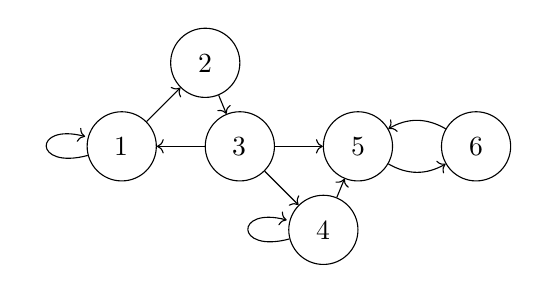
\begin{tikzpicture}[->,auto,node distance=1.5cm]
    \node[state] (1) {\(1\)};
    \node[state,above right of=1] (2) {\(2\)};
    \node[state,right of=1] (3) {\(3\)};
    \node[state,below right of=3] (4) {\(4\)};
    \node[state,right of=3] (5) {\(5\)};
    \node[state,right of=5] (6) {\(6\)};

    \draw
    (1)
    edge[loop left] node{} (1)
    edge[] node{} (2)
    (2)
    edge[] node{} (3)
    (3)
    edge[] node{} (1)
    edge[] node{} (4)
    edge[] node{} (5)
    (4)
    edge[loop left] node{} (4)
    edge[] node{} (5)
    (5)
    edge[bend right] node{} (6)
    (6)
    edge[bend right] node{} (5);
  \end{tikzpicture}
  \end{center}
\end{minipage}
  has communicating classes \(\{1,2,3\}, \{4\},\{5,6\}\), only the last of which is closed.
\end{eg}

\section{Recurrence \& Transience}

\subsection{Definition}

Introduce notation \(\prob_i(\cdot) = \prob(\cdot| X_0 = i), \E_i(\cdot) = \E(\cdot|X_0=i)\).

\begin{definition}
The \emph{first-passage time} of \(j\in S\) is
\[
T_j = \min \{n\geq 1: X_n=j\}.
\]
The \emph{first-passage probability} are
\[
f_{i,j}(n) = \prob_i(T_j=n).
\]
\end{definition}

\begin{definition}
  \(i\in S\) is \emph{recurrent (or persistent)} if
  \[
\prob_i(T_i < \infty) = 1,
  \]
  and \emph{transient} otherwise.
\end{definition}

\subsection{Recurrent Condition}

\begin{theorem}
  \label{thm:recurrent}
  \(i\) is recurrent if and only if
  \[
    \sum_{n\geq0}^{}p_{i,i}(n) = \infty.
  \]
\end{theorem}

Before we prove the theorem, introduce two generating functions:
\begin{align*}
  P_{i,j}(s) &= \sum_{n\geq0}^{ }p_{i,j}(n)s^n \\
  F_{i,j}(s) &= \sum_{n\geq0}^{ }f_{i,j}(n)s^n
\end{align*}
with the convention that
\begin{align*}
  p_{i,j}(0) &= \delta_{i,j} =
                 \begin{cases}
                   1 & i = j \\
                   0 & i \neq j
                 \end{cases}\\
  f_{i,j}(0) &= 0 \, \forall i,j
\end{align*}

Note that
\begin{align*}
  p_{i,j}(n) &= \sum_{m=1}^{n}\prob_i(X_n=j|T_j=m)\prob_i(T_j=m) \\
             &\stackrel{\text{MP}}{=} \sum_{m=1}^{n}p_{j,j}(n-m)f_{i,j}(m)
\end{align*}
which is the convolution of \(p\) and \(f\).

It follows that for \(n\geq 1\),
\begin{align*}
  \sum_{n\geq1}^{ } p_{i,j}(n)s^n &= \sum_{n\geq1}^{ } \sum_{m=1}^{n} \Big( f_{i,j}(m)s^m \Big) \Big(p_{j,j}(n-m)s^{n-m} \Big) \\
  P_{i,j}(s) -\delta_{i,j} &= \sum_{m=1}^{\infty} \sum_{n=m}^{\infty} \Big( f_{i,j}(m)s^m \Big) \Big(p_{j,j}(n-m)s^{n-m} \Big) \\
                                  &= \sum_{m\geq1}^{ } f_{i,j}(m)s^m \sum_{r\geq0}^{} p_{j,j}(r)s^r \\
                                  &= F_{i,j}(s) P_{j,j}(s)
\end{align*}
be careful when dealing with double summations.

\begin{theorem}
  \[
    P_{i,j}(s) = \delta_{i,j} + F_{i,j}(s)P_{j,j}(s) \text{ for } |s| < 1.
  \]
\end{theorem}

The \(|s| < 1\) condition: since \(|F_{i,j}(s)| < \infty\) if \(|s| < 2\),
\[
  |P_{i,j}(s)| \leq \sum_{n}^{ }|s|^n < \infty 
\]

A lemma from analysis before we finally prove Theorem~\ref{thm:recurrent}:
 \begin{lemma}[Abel's Lemma]
  Let \((u_i)_{i\geq0}\) be a non-negative sequence such that
  \[
    \mathcal U(s) = \sum_{i=0}^{\infty}u_is^i
  \]
  converges when \(|s| <1\), then
  \[
    \sum_{i=0}^{\infty}u_i = \lim_{s\to 1^-} \mathcal U(s),
  \]
  whether or not this limit is finite.
\end{lemma}

\begin{proof}
  Exercise.
\end{proof}

\begin{proof}[Proof of Theorem~\ref{thm:recurrent}]
  For \(|s| < 1\), then
  \begin{align*}
    p_{i,i}(s) &= 1+ F_{i,i}P_{i,i} \\
    P_{i,i} &= \frac{1}{1-F_{i,j}}
  \end{align*}
Let \(s \to 1^-\), then by Abel's Lemma
\begin{equation}
  \label{eqn:recurrent P}
  P_{i,i}(1) = \infty \Leftrightarrow F_{i,i}(1) =1
\end{equation}
i.e. \(i\) is recurrent.
\end{proof}

\subsection{Properties of Recurrence}

\begin{theorem}[Recurrence as a class property]
  Let \(C\) be a communicating class, then
  \begin{enumerate}
  \item either every state in \(C\) is recurrent or every state is transient,
  \item if \(C\) contains some recurrent state then \(C\) is closed.
  \end{enumerate}
\end{theorem}

\begin{proof}\leavevmode
  \begin{enumerate}
  \item Let \(i,j \in C\), \(i \neq j\). There exist \(m,n\geq 1\) such that
    \[
      \alpha = p_{i,j}(m)p_{j,i}(n) >0.
    \]
    This is simply a restatement of the communicating property. Then
    \begin{align*}
      p_{i,j}(m+k+n) \geq p_{i,j}(m)p_{j,j}(k)p_{j,i}(n) = \alpha p_{j,j}(k)
    \end{align*}
    Intuitively, the middle term is the probability of going from \(i\) to \(i\) by passing \(j\) at step \(m\) and \(m+k\).
    Thus
    \[
      \sum_{k}^{}p_{i,i}(m+k+n) \geq \alpha \sum_{k}^{ }p_{j,j}(k).
    \]
    Thus \(j\) recurrent implies that \(i\) is recurrent. Vice versa.
  \item Suppose \(i\in C\) is recurrent but \(C\) is not closed. Then there exists \(j\in C, k\notin C\) with \(p_{j,k} > 0\). By the previous part \(j\) is recurrent so
    \[
      1 = \prob_j(T_j < \infty) = 1 - \prob_j(\text{no return to } j) \leq 1- p_{j,k} < 1
    \]
    Absurd.
  \end{enumerate}
\end{proof}

\begin{theorem}
  \label{thm:recurrent irreducible chain}
  Assume \(|S| < \infty\), then
  \begin{enumerate}
  \item \(S\) contains some recurrent state,
  \item if the chain is irreducible, all states are recurrent.
  \end{enumerate}
\end{theorem}

Similar as before, we need a proposition before the proof:
  \begin{proposition}
    If \(j\) is a transient state then
    \[
      \forall i,\, p_{i,j}(n) \to 0 \text{ as } n\to\infty
    \]
  \end{proposition}

  \begin{proof}
    Asuume \(j\) is transient. By \eqref{eqn:recurrent P},
    \[
      P_{j,j}(1) < \infty.
    \]
    By Theorem~\ref{thm:recurrent},
    \[
      \sum_{n}^{ }p_{i,j}(n) = P_{i,j}(1) < \infty
    \]
    so \(n\)th term \(p_{i,j}(n)\) tends to \(0\) as \(n\to \infty\).
  \end{proof}

\begin{proof}\leavevmode
  \begin{enumerate}
  \item \(\sum_{j\in S}^{ }p_{i,j}(n) = 1 \) since \(P\) is a stochastic matrix. If \(j\) is transient then each summand tends to \(0\) as \(n\to \infty\), which is absurd since \(|S| < \infty\).
  \item Obvious.
  \end{enumerate}
\end{proof}

\subsection{Random Walks and Pólya's Theorem}

In this section, we discuss simple symmetric random walk on \(d\)-dimensional lattices, i.e.\ \(\Z^d\), in particular answering the question when the chain is recurrent.\footnote{Note that this chain is irreducible so by Theorem~\ref{thm:recurrent irreducible chain} either we can talk about recurrence as a chain property.}  It turns out that there is a surprisingly beautiful result.

We call two points \(x\) and \(y\) \emph{neighbours} if
\[
  \sum_{i}^{ }|x_i-y_i| = 1,
\]
i.e.\ they differ by \(1\) in only one coordinate. Let \(X\) be a symmetric random walk on \(\Z^d\) where \(d \geq 1\), i.e.\ \(X = (X_1, X_2, \dots)\) is a Markov chains with state space \(S = \Z^d\) and transition probability
\[
  \prob(X_{n+1} = y | X_n = x) =
  \begin{cases}
    0 & \text{ if } x \text{ and } y \text{ are not neighbours} \\
    \frac{1}{2d} & \text{ if } x \text{ and } y \text{ are neighbours}
  \end{cases}
\]

\begin{theorem}[Pólya's]
  \(X\) is recurrent if \(d \leq 2\) and transient if \(d \geq 3\).
\end{theorem}

\begin{proof}
  First set \(d = 1\). Recall that \(0\) is recurrent if and only if \(\sum_n p_{0,0}(n) = 0\). However, it is not possible to return to the same place after an odd number of steps so the expression simplifies to
  \begin{equation}
    \label{eqn:polya}
    \sum_n p_{0, 0}(2n)
    \tag{\(\ast\)}
  \end{equation}
  In the even case, the random walk returns to \(0\) if and only if there are equal number of movement to either direction so by applying the binomial distribution,
  \[
    p_{0,0}(2n) = \left( \frac{1}{2} \right)^{2n} \binom{2n}{n}
  \]
  To simplify this, recall Sterling's formula
  \[
    n! \sim \left( \frac{n}{e} \right)^n \sqrt{2\pi n} \text{ as } n \to \infty.
  \]
  So
  \[
    p_{0,0}(2n) \sim \frac{1}{\sqrt{\pi n}}
  \]
  and the sum~\eqref{eqn:polya} tend to infinity.

  Now let \(d = 2\). By the same reasoning and generalising binomial to multinomial coefficients, we get
  \begin{align*}
    p_{0,0}(2n) &= \left( \frac{1}{4} \right)^{2n} \sum_{m=0}^{n} \binom{2n}{m, m, n-m, n-m} \\
                &= \left( \frac{1}{4} \right)^{2n} \sum_{m=0}^{n} \frac{(2n)!}{(m!)^2 ((n-m)!)^2} \\
                &= \left( \frac{1}{4} \right)^{2n} \frac{(2n)!}{(n!)^2} \sum_{m=0}^{n} \binom{n}{m} \binom{n}{n-m} \\
    \intertext{Now pause and think: the summation represents the number of ways to take \(m\) balls from a bag of \(n\) balls and take \(n-m\) balls from another bag of \(n\) balls, for \(0 \leq m \leq n\), but this is precisely the number of ways to take \(n\) balls from \(2n\) balls!}
                &= \left( \frac{1}{4} \right)^{2n} \binom{2n}{n} \binom{2n}{n} \\
                &= \left( p_{0,0}^{d=1}(2n) \right)^2
  \end{align*}
  thus the sum~\eqref{eqn:polya} also tends to infinity and \(0\) is recurrent.

  Let \(d = 3\) (similar for \(d \geq 4\)) and we have
  \begin{align*}
    p_{0,0}(2n) &= \left( \frac{1}{6} \right)^{2n} \sum_{i+j+k = n} \binom{2n}{i,i,j,j,k,k} \\
                &= \left( \frac{1}{6} \right)^{2n} \sum_{i+j+k = n}^{}\frac{(2n)!}{(i! j! k!)^2} \\
                &= \left( \frac{1}{6} \right)^{2n} \binom{2n}{n} \sum_{i+j+k = n}^{} \left( \frac{n!}{i! j! k!} \right)^2 \\ 
                &=  \left( \frac{1}{2} \right)^{2n} \binom{2n}{n} \sum_{i+j+k = n}^{} \left( \frac{n!}{3^n i! j! k!} \right)^2 \\
                &\leq \left( \frac{1}{2} \right)^{2n} M_n \sum_{i+j+k = n}^{}\frac{1}{3^n i! j! k!} \\
    \intertext{ where \(M_n = \max \{ \frac{n!}{3^n i!j!k!}, i+j+k = n \} \).}
    \intertext{The reason we introduce \(3^n\) becomes apparent in this step: \( \frac{n!}{3^n i! j! k!}\) is the probability of, upon throwing \(n\) balls into \(3\) urns, finding \(i, j, k\) in each respectively. Thus they sum up to \(1\).}
                &\leq \left( \frac{1}{2} \right)^{2n} \binom{2n}{n} \frac{n!}{3^n \left( \floor{n/3}! \right)^3}
  \end{align*}
  The upper bound of \(M_n\) is left as an exercise. By Sterling's formula,
  \[
    p_{0,0}(2n) \leq \frac{C}{n^{3/2}}
  \]
  so the sum is finite and \(0\) is recurrent.
\end{proof}

We have seen that the probability \(p_{0, 0}(2n)\) when \(d = 2\) is the square of the probability when \(d = 1\), but when \(d = 3\) it doesn't become cubed. It should inspire us to suspect that the \(d = 2\) case is simple enough such that the random walks in two directions are ``independent'', but when \(n \geq 3\) there is some hidden structure that destroys such independence. What is so special about dimension two?

There is an alternative way to tackle this problem that might be more lucid and shed some light on the magical property of \(d = 2\). Instead of cartesian coordinates \(X_n = (A_n, B_n)\), rotate the axes by \(45^\circ\) clockwise. The new coordinates, scaled by a constant factor for convenience, are
\[
  Y_n =
  \begin{pmatrix}
    U_n \\
    V_n
  \end{pmatrix}
  = \sqrt 2
  \begin{pmatrix}
    \cos 45^\circ & -\sin 45^\circ \\
    \sin 45^\circ & \cos 45^\circ
  \end{pmatrix} X_n
  =
  \begin{pmatrix}
    A_n - B_n \\
    A_n + B_n
  \end{pmatrix}
\]
\iffalse
\begin{align*}
  U_n &= A_n - B_n \\
  V_n &= A_n + B_n \\
  Y_n &= (U_n, V_n)
\end{align*}
\fi

Claim \(U = (U_n)\) and \(V = (V_n)\) are \emph{independent} random walks on \(\Z\):

\begin{proof}
  \begin{align*}
    \prob(Y_{n+1} &= Y_n+ (1,1)) = \prob(X_{n+1} = X_n + (1,0)) = \frac{1}{4} \\
                  &= \prob(U_{n+1} - U_n = 1, V_{n+1} - V_n = 1)
  \end{align*}
  since during one step \(X_n\) can only change by \(1\) in one coordinate. Similar for the other three cases.

  So
  \[
    \prob(U_{n+1} - U_n = \alpha, V_{n+1} - V_n = \beta) = \left( \frac{1}{2} \right)^2 = \prob(U_{n+1} - U_n = \alpha) \prob(V_{n+1} - V_n = \beta)
  \]
  for \(\alpha, \beta = \pm 1\). \(U_n\) and \(V_n\) are independent and each generates a random walk on \(\Z\).
\end{proof}

By independence
  \[
    \prob_0(X_n = (0,0)) = \prob_0(Y_n = (0,0)) = \prob_0(U_n = 0) \prob_0(V_n = 0)
  \]
  so
  \[
    p_{0,0}^{d=2}(2n) = \left( p_{0,0}^{d=1} \right)^2.
  \]

  The moral of this calculation is, two dimensional random walk is indeed the product of two one dimensional cases, but in a not-entirely-straightforward way.

\iffalse
\appendix

\section{Resources}


Reading list: Probability, an introduction Grimmet, Welsh, 2nd edition, Chapter 12

%webpage: www.statslab.cam.ac.uk/~grg/
\fi
\end{document}